\documentclass{article}

\usepackage[utf8]{inputenc}
\usepackage[margin=2cm,nohead]{geometry}
\usepackage{graphicx}

\setlength{\parindent}{0pt}

\begin{document}

\section*{IT19tb WIN7 S4 Aufgabe 1}
Leo Rudin \& Stefan Teodoropol

\subsection*{a)}

Auswahl möglicher Fixpunktgleichungen für Ursprungsfunktion: \( f(x) = 230x^4 + 18x^3 + 9x^2 - 221x - 9 \)\\\\
\( F1(x) = \frac{230x^4 + 18x^3 + 9x^2 - 9}{221} \)\\
\( F1'(x) = \frac{920x^3}{221} + \frac{54x^2}{221} + \frac{18x}{221} \)\\\\
\( F2(x) = \sqrt{\frac{230x^4 + 18x^3 - 221x - 9}{-9}} \)\\
\( F2'(x) = \frac{1}{2} * \frac{1}{\sqrt{\frac{230x^4+18x^3-221x-9}{-9}}} * \frac{920x^3+54x^2-221}{-9} \)\\\\
Für \( \overline{x}_1 \) wählen wir den Startwert \( -0.1 \):\\
\( |F1'(-0.1)| = 0.00986425339366516 < 1 \)\\
Somit wird der Punkt für den Startwert -0.1 konvergieren.\\\\
Fixpunktiteration für Startwert -0.1:\\
\( F1(-0.1) = -0.04029411764705882.. \)\\
\( F1(-0.04029411764705882..) = -0.040660446815532846.. \)\\
\( F1(-0.040660446815532846..) = -0.0406592846229974.. \)\\
\( F1(-0.0406592846229974..) = -0.0406592883275295.. \)\\\\
\( \overline{x}_1 \approx -0.04065928... \)\\\\
Für \( \overline{x}_2 \) wählen wir den Startwert 0.9:\\
\( |F1'(0.9)| = 3.305972850678734 > 1 \)\\
\( |F2'(0.9)| = 12.4153 > 1 \)\\
Wir schliessen daraus, dass wir auf dem Interval \( [0,1] \) für den Startwert 0.9 keine Fixpunktiteration ausführen können, da die Steigung an dieser Stelle zu gross ist und die Fixpunktiteration nicht konvergiert bzw. der Fixpunkt ist nicht anziehend.

\newpage

\subsection*{b)}

Für die erste Bedingung \( [a,b] \rightarrow [a,b] \), das heisst die Funktion F1(x) bildet sich auf das gleiche Interval ab, haben wir gezeigt, indem wir die Funktion geplottet haben und die Funktionswerte betrachten:
\begin{figure}[h!]
\centering
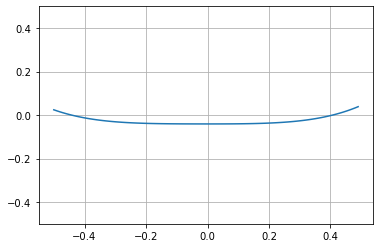
\includegraphics[scale=1]{plot_aufg1b.png}
\caption{Plot für F1(x) zwischen -0.5 und 0.5 auf x und y-Achse.}
\label{fig:plot_aufg1b.png}
\end{figure}

Dann rechnen wir \( \alpha \) aus, indem wir den in der Aufgabenstellung vorgegebenes Maximum in die Ableitung einsetzen und kriegen dann:

\[ \alpha = F1'(0.5) = 0.6221719457013575 \]

\( \alpha \) erfüllt somit die Bedingnung \( 0 > \alpha > 1 \). Das heisst alle Bedingungen des Banachscher Fixpunktsatzes sind erfüllt.

\subsection*{c)}

Wir nutzen folgende Formel für die Fehlerabschätzung:\\
\( |x_n - \overline{x}| \leq \frac{\alpha^n}{1-\alpha} |x_1 - x_0| \)

Für \( |x_n - \overline{x}| \) setzen wir \( 10^{-9} \) ein und für \( \alpha \) unseren vorherigen errechnet Wert:\\\\
\( 10^{-9} \leq \frac{0.62^n}{0.38} * |F(-0.1) - (-0.1)| \)\\
\( 10^{-9} \leq \frac{0.62^n * 0.05970588235294118}{0.38} \)\\
\( 6.3645320197044331213084520371764 * 10^{-9} \leq 0.62^n \)\\
\( log(6.3645320197044331213084520371764 * 10^{-9}) \leq log(0.62^n) \)\\
\( log(6.3645320197044331213084520371764 * 10^{-9}) \leq n * log(0.62) \)\\
\( \frac{log(6.3645320197044331213084520371764 * 10^{-9})}{log(0.62)} \leq n \)\\\\
\( n \geq 39.4793.. \)\\\\
Somit ist unsere Abweichung kleiner als \( 10^{-9} \) wenn wir n grösser als 39.3793 wählen. Wir wählen also die nächstgrössere Zahl n = 40.


\end{document}
